% More motivated proof of summation by parts
% cyclic permutation

%%% (CPT comments)
% Move  section "common sums" before "iterated sums"
% Add new section -- Matrix multiplication. Show how matrix multiplication is represented in summation notation.  Use to prove that (AB)^T = B^T A^T.  Introduce trace of a matrix, and prove that trace(AB) = trace(BA)  (when AB is square)  Exercise:  show that trace(ABC) = trace(CAB)
% Introduce epsilon symbols (from physics), and relate to determinant of $3\times 3$ matrix, and to vector cross product.  Show the BAC - CAB rule (I can show you this)
% Add new section -- summation by parts
% Derive formula (Look at http://en.wikipedia.org/wiki/Summation_by_parts in method section)
% Do example  sum of i^2
% exercises:  sum of i^3, sum of (i)*2^i

%If its not already included, it would be useful to have a list of identities involving summation notation. JW

\chap{Sigma Notation}{Sigma}
We are about to start looking at polynomials, which means we will be working with sums of terms -- sometimes many terms. Such sums are often written using \emph{Sigma notation}.  It's possible that you are already a master of Sigma notation. If not, you can brush up with the material in this section. (At very least, you should try some of the exercises to make sure that you haven't gotten rusty!)\footnote{This chapter was written by David Weathers and Johnny Watts (edited by CT).}

\section{Lots of examples}

It's unavoidable that in mathematics, one often encounters sums.  Sometimes these sums have very few terms, but occasionally the sums can reach hundreds, thousands or even an infinite number of terms.  In these cases, rather than listing each and every term or listing the first several terms and assuming the pattern is obvious, one can represent a sum using \emph{summation notation}\index{Summation notation}, often referred to as \emph{Sigma notation}\index{Sigma notation}. 

 Sigma notation has four main parts:  the \emph{index variable}, the \emph{starting value}, the \emph{final value} and the \emph{formula}.
These parts are illustrated in the following example.

\begin {example}{Sigma1}
Consider:
\[\sum _{i=1}^{10}(i+2)\]
In this case, the $\Sigma$ symbol lets us know that this is a sum.  The $i=1$ serves two functions.  It tells us that the index variable is $i$, and that $i$ has a starting value of 1. The $10$ is the final value, and the $(i+2)$ to the right of the $\Sigma$ is the formula. The $i$ in the formula, takes each integer value from the starting value (1) to the final value (10).  
Therefore we have:
% For each possible integer value $i$ in the inclusive range from start value to final value, we plug in that value into the formula to get a term.  Then, as per the summation, we add all the terms together.  Therefore:
\[\sum _{i=1}^{10}(i+2) = 3 + 4 + 5 + 6 + 7 + 8 + 9 + 10 + 11 + 12=75.\]
%With a few small changes, we can alter the sum dramatically.  
\end {example}

This notation has a lot of flexibility. For example, the sum's formula can be a constant value:
\[\sum _{i=1}^{10}5 = 5 + 5 + 5 + 5 + 5 + 5 + 5 + 5 + 5 + 5 = 50.\]
Or we could have the index as an exponent:
operator value
\[\sum _{i=1}^{10}(2^i) = 2^1 + 2^2 + 2^3 + 2^4 + 2^5 + 2^6+ 2^7+ 2^8+ 2^9+ 2^{10} \]
Now all the examples so far have a numerical value that can be calculated.  However, summation notation can also be used to express functions of variables such as:  
\[\sum _{i=1}^{10}(x^i)= x^1 + x^2 + x^3 + x^4 + x^5 + x^6+ x^7+ x^8+ x^9+ x^{10} \]
Note that any variables in the formula that do not match the index are left as variables (such as $x$ in the previous example).  
While we do not know what the sum value is other than in terms of $x$, we can much more concisely state the sum in Sigma notation.

Another typical use for the index in the formula is to denote an index in a coefficient.  Consider the polynomial:
\[ax^2 + bx + c.\]
Instead of using a different letter, we can use a subscript to denote a different value but use the same letter:
\[a_2x^2 + a_1x + a_0.\]
And when we use subscripts, we can use the index in the formula to denote that subscript.
\[\sum_{i=0}^{2}a_ix^i\]
% \noindent In this last example, we not only changed the formula, but we also changed the starting and final values.  Note what happens  If we change the starting value or ending condition, 

Changing the starting and/or final values does not affect the pattern of the formula, but it does change the number of terms and any index values used in that formula.  Take one of the previous examples:
\[\sum _{i=1}^{10}i = 1 + 2 + 3 + 4 + 5 + 6 + 7 + 8 + 9 + 10\]
If we were to change the $i=1$ to $i=4$ then the sum would lose terms 1,2,3:
\[\sum _{i=4}^{10}i = 4 + 5 + 6 + 7 + 8 + 9 + 10\]
Likewise, if we were to also change the 10 to 6, it would lose the terms 10,9,8 and 7;
\[\sum _{i=4}^{6}i = 4 + 5 + 6.\]

\begin{exercise}{Sigma Notation Practice}
%Calculate the following sums and combine like terms.
Evaluate the following:
%%% Change so that sums are in display format. The summation indices are too cramped, and the fraction is too small.
\begin {enumerate}[(a)]
\item
$\displaystyle{\sum _{i=0}^{400} \,2}$
\item
$\displaystyle{ \sum_{j=17}^{20} \, 2j^2 - j}$
\item
$\displaystyle{ \sum_{k=0}^{4}(x^{2k} - k)}$  \quad (Your answer should be in terms of  $x$).
\item
$\displaystyle{ \sum_{k=0}^{7} (-1)^k\frac{x^{k}}{(k+1)(k+2)}}$ \quad  (Your answer should be in terms of $x$).
\end {enumerate}
\end{exercise}

\section{Sigma notation properties}

% Sigma, as with any other math notation, is designed not only to offer control and concise notation, but to offer the ability to change the representation of that notation without changing the value.  There are some circumstances where numbers can be moved or removed from the sum and yet the sum maintains the same value.  
As with any algebraic notation, there are rules that allow us to do algebraic manipulations with expressions that involve Sigma. 
Take for example:
\[\sum_{i=0}^{5}2i\]
We know this is the Sigma notation for $2\cdot1+2\cdot2+2\cdot3+2\cdot4+2\cdot5$. Using the distributive property of addition and multiplication of integers, we know this sum is the same as $2\cdot(1+2+3+4+5)$.  Now we convert the sum in the parenthesis to Sigma notation to yield
\[2\cdot\sum_{i=0}^{5}i.\]
The same argument could be used for any sum  multiplied by any constant. We can write this rule as:
\[\sum_{i=a}^{b} c \cdot d_i = c \cdot \sum_{i=a}^{b}  d_i,\]
where $c$ denotes an arbitrary constant and $d_i$ represents the term of the sum corresponding to index $i$.
%If one were to substitute any real number for 2, the same math could be shown.  The only exception is in the case of $0$ being the constant multiple in which case the sum is $0$ and the distribution would require division by $0$. 
%%% Need to give additional sum rules:  sum (x_i + y_i), sum (c*x_i + d*y_i)
Some additional sum rules:
\[ \sum_{i=0}^n \left(x_i +y_i \right) = \sum_{i=0}^n x_i + \sum_{i=0}^n y_i \]
\[ \sum_{i=0}^n \left(c \cdot x_i + d \cdot y_i \right) = c \cdot \sum_{i=0}^n x_i + d \cdot \sum_{i=0}^n y_i \]

It is also possible to shift 
%some addition and subtraction from the formula to 
the starting and final values without changing the value of the formula. Take the following sum:
\[\sum_{i=2}^{7}(i-1)\] 
In this case, the sum is
%index $i$ starts at 2 and ranges to 7 with each value being subtracted by 1.  This in effect gives us 
$1+2+3+4+5+6$, which can be represented as:
\[\sum_{i=1}^{6}i\] 
%This can even be used when the index in the formula is being affected by another function.
%Or in general, \sum_{n=j}^k f(n) = \sum_{n=j+p}^{k+p} f(n-p) JW
A similar example is:
\[\sum_{i=2}^{4}(i+1)(i+2)=(2+1)(2+2) + (3+1)(3+2)+(4+1)(4+2) = 62\]
 \[(3+0)(3+1) + (4+0)(4+1)+(5+0)(5+1) = \sum_{j=3}^{5}j(j+1).\] 
%Notice that whenever the index and ending condition change, it must change all instance of the index in the formula. Another way to think about it, is substituting a new index into the whole summation. Given:
Changing the starting and final values in this way can be thought of as a change of variable. For instance, in the previous example we had
\[\sum_{i=2}^{i=4}(i+1)(i+2).\]
Let $j = i+1$, and solve for $i$: $i = j-1$. We then replace all $i$'s in the formula with $j-1$ to obtain
% Then with $i=2$ add 1 to each side to get $ i+1 = 3$ with $i=4$ add 1 to each side to get $ i+1 = 5$ with $i+2$ separate into $i+1+1$ then substitue $j$ for each $i+1$ to yield.
\[\sum_{(j-1)=2}^{(j-1)=4}((j-1)+1)((j-1)+2),\]
and after algebraic simplification we get
\[\sum_{j=3}^{5}j(j+1),\]
as before.

Occasionally, it may be necessary to add or remove a single term from the sum.  This can be done by changing the start value or end condition.The following example illustrates this, as well as demonstrating some of our summation manipulation rules:
\[\sum_{i=1}^{10}i = 1 + \sum_{i=2}^{10} i = 1+ \sum_{i=1}^9 ( i+1) = 1 +  \sum_{i=1}^9  i +  \sum_{i=1}^9  1 =  \sum_{i=1}^9  i + 10.\]
When removing a term from the middle, it may be necessary to split the sum into two separate sums.
\[\sum_{i=1}^{10}i = \sum_{i=1}^{3}i + 4 + \sum_{i=5}^{10}i.\]
%However adding a term to a sum can be quite difficult.  The formula has to account for the new term which is not always possible.  Take for example the sum off odd numbers from 1 to 51.
%\[\sum_{i=0}^{25}(2i+1)  \]
%If it were necessary to add the number 2 to the sum, it would not be possible to merely change the parameters of Sigma to include 2.  In this case it is better to leave the notation as :
%\[2 + \sum_{i=0}^{25}(2i+1)  \]

%insert exercises for sigma notation modification
\begin {exercise}{}
Take the following Sigma notation examples and change the formula and final value so that the starting value becomes 0 and the sum maintains the same value.  Calculate the value of both the listed sum and the resulting sum to show that the value is the same.
\begin {enumerate} [(a)]
 \item
$\displaystyle{\sum_{i=3}^{46}2i}$
\item
$\displaystyle{\sum_{j=7}^{20}\cos(j\pi )}$
\item
$\displaystyle{\sum_{j=20}^{40}j-20}$
\end {enumerate}
\end{exercise}

\begin {exercise}{}
We have shown that a ``sum rule'' holds for sigma notation.  Is there a corresponding ``product rule''? That is: is it true that
\[ \sum_{i=0}^n x_i y_i \stackrel{?}{=} \left(\sum_{i=0}^n x_i \right) \left(  \sum_{i=0}^n y_i \right). \]
If true then prove it; if not, give a counterexample.
\end{exercise}


\section{Nested Sigmas}
Since any  sufficiently patterned summation can be replaced with Sigma notation, it's quite possible for one Sigma to end up inside another:

\[\sum_{i=0}^{3}\left( \sum_{j=0}^{2}1\right)\]

This means that for each value of the index of the outside Sigma, the entire sum of the inside Sigma must be calculated.  In this case, $\sum_{j=0}^{2}(1)=3$, so we have

\[\sum_{i=0}^{3}\left( \sum_{j=0}^{2}1\right) =  \sum_{i=0}^{3}\ 3  = 3+3+3+3 = 12. \]

The situation becomes more interesting when the sum inside depends on the the index variable of the outside Sigma:

\[\sum_{i=0}^{3}\left(\sum_{j=0}^{i}1\right)\]

Unlike the previous case, the inside sum will change depending on what $i$ is.  When $i=0$ then $\sum_{j=0}^{i}1=\sum_{j=0}^{0}1=1$ so 1 would be the first term in the outside sum.  When $i=1$ then $\sum_{j=0}^{i}1=\sum_{j=0}^{1}1=1+1=2$ so 2 would be the next term.  With each successive term, the inside sum increases by 1, so the result is $1+2+3+4 = 10$.

 Note that the index of the outer sum may appear in any or all parts of the inner sum. Here are some examples:  

\[\sum_{i=0}^{3} \left(\sum_{j=i}^{10}1\right); \qquad
\sum_{i=0}^{3} \left(\sum_{j=1}^{10}i \right); \qquad
\sum_{i=0}^{3}\left(\sum_{j=i}^{2i}3i+x^j\right).\]

When using nested sums, it is possible to rearrange the order of summation.  Take for example:
\[\sum_{i=0}^{2} \left( \sum_{j=0}^{i}1 \right)\]
The first term has $i=0$ and $j=0$: we write this as $(i,j)=(0,0)$. When $i=1$, then we have two terms:  $j=0$ and $j=1$. Finally, when $i=2$, we have $j=0,1,$ or 2.  Altogether we have the index pairs: $(0,0), (1,0), (1,1), (2,0), (2,1), (2,2)$. These index pairs may be displayed on a grid, as shown in Figure~\ref{fig:summation1}.
\begin{figure}[htb]
\begin{center}
	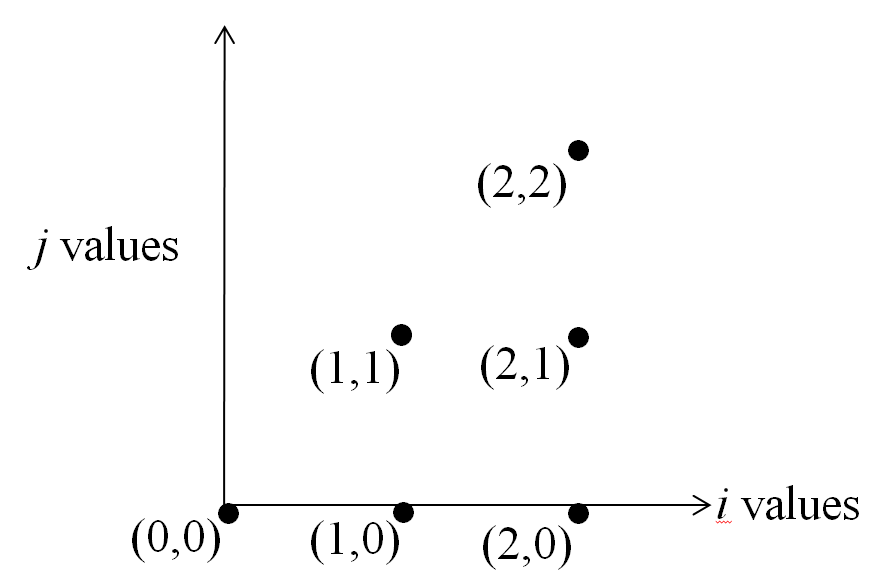
\includegraphics[width=3.0in]{images/i02j0igraph.png}
\caption{\label{fig:summation1} Grid points corresponding to the terms in the sum: $ \sum_{i=0}^{2} \left( \sum_{j=0}^{i}1 \right)$.}
\end{center}
\end{figure} 

Alternatively, we can arrange these index pairs by $j$ coordinate.  When $j$ is 0, $i$ takes the values (0,1,2), when $j$ is 1, $i$ takes the values of (1,2) and when $j$ is 2 $i$ takes the value 2.  This can be expressed as the sum:
\[\sum_{j=0}^{2} \left(\sum_{i=j}^{2}i \right)\]

So far our examples have only two Sigmas, but it's quite possible to have an unlimited number of nested Sigmas. For example, with three nested Sigmas we would have grid points in three dimensions.  It doesn't matter what order you sum the terms in--as long as you include them all!

%Another handy identity for more than one index:JW
%\sum_{i=n}^s \sum_{j=m}^t a_{i,j} = \sum_{j=m}^t sum_{i=n}^s a_{i,j} 
\begin {exercise}{}
Rewrite each of the following nested sums, exchanging the order of sums and changing the start values and end conditions as needed so that the nested sum maintains the same value. (In some cases, drawing a grid point diagram similar to Figure~\ref{fig:summation1} may be helpful.)
\begin {enumerate}[(a)]
\item
$\displaystyle{\sum_{i=0}^{4}\left(\sum_{j=0}^{8}i\right)}$
\item
$\displaystyle{\sum_{j=0}^{2}\left( \sum_{i=j}^{2j}i+j\right)}$
\item
$\displaystyle{\sum_{k=0}^{17}\left(\sum_{i=0}^{2k}2i+1 \right)}$
\item
$\displaystyle{\sum_{i=1}^{10}\left(\sum_{j=i}^{i} (i-j) \right)}$
\item
$\displaystyle{\sum_{i=1}^{10}\left(\sum_{j=i}^{10} ij \right)}$
\item
$\displaystyle{\sum_{i=m}^{n}\left(\sum_{j=i}^{p}jx^i \right)}$
\item
$\displaystyle{\sum_{i=m}^{n}\left(\sum_{j=q}^{i}(i-j)^2 \right)}$
\end {enumerate}
\end{exercise}

\begin{exercise}{}
Using exchange of summation and other sum manipulation techniques, find the exact values of the following sums:
\begin{enumerate}[(a)]
\item
$\displaystyle{\sum_{i=1}^{10} \sum_{j=1}^{10} (j-i)}$
\item
$\displaystyle{\sum_{i=1}^{10} \sum_{j=1}^i \frac{1}{11-j}}$
\item
$\displaystyle{\sum_{i=1}^{10} \sum_{j=1}^i \frac{i}{j}}$
\item
$\displaystyle{\sum_{i=1}^{10} \sum_{j=1}^i (j+i)}$
\end{enumerate}
\end{exercise}

\section{Common Sums}
There are several sums, even a few infinite sums, that the total value is known. One very basic example is:
\[\sum_{i=1}^{k}1\]
The answer is NOT 1. (What is it?) Make sure you don't get tripped up by this one.

Another very useful example is:

\[\sum_{i=1}^{k}i=1+2+3\cdots+(k-1) + k\]

If one were to take the first term 1 and add it to the last term $k$, we get $k+1$.  If we take the second term 2 and add to the second-to-last term $k-1$ again we get $k+1$.  This is true for all terms in between.  In the case of an even number of terms (such as $1+2+3+4$),  the terms split evenly.  In the case of an odd number of terms (such as $1+2+3+4+5+6+7$) we have 3 pairs that add to 8 but an additional term in the middle.  In either case, we take the first term add to the last term and multiply that quantity by 1/2 the number of terms.  The formula is thus:

\[\sum_{i=1}^{k}i= \frac{k(k+1)}{2}.\] 

We can use the same reasoning to arrive at the following formula.

\[\sum_{i=a}^{k}i=a+(a+1)+(a+2)\cdots+(k-1) + k = (k+a)*(k-a+1)/2,\] 
where $a$ and $k$ are integers and $a<k$.

%%% Need a better example before these exercises. Students don't know how to represent an odd number.  You can also do exercises where you skip 3 numbers instead of 2
\begin {exercise}{}
\begin {enumerate}[(a)]
\item 
Write the sum of odd integers from $2a+1$ to $2k+1$ in Sigma notation.
\item
Give a formula for the sum that you wrote in (a).  (Use the same reasoning that we used to find sums of consecutive integers.)
\item 
Write the sum of even integers from $2a$ to $2k$ in Sigma notation.
\item
Give a formula for the sum that you wrote in (c). 
\item 
Write the sum of every $5^{\text{th}}$ integer from $a$ to $a + 5k$ in Sigma notation.
\item
Give a formula for the sum that you wrote in (e). 
\end {enumerate}
\end {exercise}

%%% Give the derivation of the geometric series for a finite number of terms.
One infinite sum called the \emph{geometric series}, and is defined as the sum of integer powers of a common base.  For example, here is the geometric series when the base is 1/2:
\[\sum_{i=0}^{\infty}\left({\dfrac{1}{2}}\right)^i=\left({\dfrac{1}{2}}\right)^0+\left({\dfrac{1}{2}}\right)^1+\left({\dfrac{1}{2}}\right)^2\cdots = 1 + {\dfrac{1}{2}} + {\dfrac{1}{4}} + {\dfrac{1}{8}}\cdots\]
As we add the terms of the sum together it becomes apparent that the total sum gets closer to 2, but never quite gets there.  However if we add all the terms together, the sum approaches:
\[\dfrac{1}{1-\dfrac{1}{2}}.\]
More generally for any value $-1<x<1$ the series:
\[\sum_{i=0}^{\infty}x^i = \dfrac{1}{1-x}\]
We can easily prove this using some fairly simple algebra.  Let $S$ be the value of this sum.  We can solve for $S$  by writing:
 \[S=1+x+x^2+x^3+ \cdots \]
\[xS=x+x^2+x^3+x^4+ \cdots \] 
Subtracting these two equations gives $S-xS=1$, and solving for $S$ gives:
\[S=\dfrac{1}{1-x}. \]
This same technique can be used to prove the formula for a geometric series with a finite number of terms:
\[ \sum_{i=0}^{n-1} ar^i = a \dfrac{1-r^n}{1-r} \]
As before, we let $S$ be the value of this sum. We then compute $S - rS$ (most terms in the sums cancel) and solve for $S$.  See if you can do this for yourself.  (It may be on the test!)

Other sums with known values include:
\[\sum_{i=0}^{\infty}\dfrac{x^i}{i!} =1+\dfrac{x^1}{1!}+\dfrac{x^2}{2!}+\dfrac{x^3}{3!} \cdots=e^x\]
\[\sum_{i=0}^{\infty}\dfrac{(-1)^i x^{2i+1}}{(2i+1)!} = \dfrac{x^1}{1!}-\dfrac{x^3}{3!}+\dfrac{x^5}{5!}\cdots= \sin(x)\]

There are also sums which \emph{diverge}\index{Sum!divergent}, that is, they can be shown to approach positive or negative infinity. Examples include:

\[\text{The harmonic series:  }\sum_{i=0}^{\infty}\left(\dfrac{1}{i} \right) \]
\[\text{The geometric series when~} |x| \ge 1: ~~\sum_{i=0}^{\infty} x^i. \]

\section{Sigma notation in linear algebra}

\subsection{Applications to matrices}

In the following discussions, we will assume that all matrices have real entries.  However, all of the results that we will prove also apply (in some cases, with slight modifications)  for matrices with \emph{complex} entries, or even matrices with entries in $\mathbb{Z}_p$.

\subsubsection*{Matrix multiplication}
It should come as no surprise that summation notation commonly shows up when working with matrices. In the following discussion, we will follow the common practice of denoting a matrix with a capital letter in italics, and the entries of the matrix with the same letter in lowercase. Thus for example, $a_{2,4}$ denotes the entry of matrix $A$ in row 2, column 4.
   
 Consider the example of multiplying the $3 \times 3$ matrix $A$ and the $3 \times 2$ matrix $B$. 
\[{A}{B} = \left( \begin{array}{ccc}
a_{1,1} & a_{1,2}  & a_{1,3}  \\
a_{2,1} & a_{2,2} & a_{2,3} \\
a_{3,1} & a_{3,2} & a_{3,3} \end{array} \right)
 \left( \begin{array}{cc}
b_{1,1} & b_{1,2}    \\
b_{2,1} & b_{2,2}  \\
b_{3,1} & b_{3,2}  \end{array} \right) \]

\[= \left( \begin{array}{cc}
a_{1,1} b_{1,1} + a_{1,2} b_{2,1} + a_{1,3} b_{3,1} & a_{1,1} b_{1,2} + a_{1,2} b_{2,2} + a_{1,3} b_{3,2}  \\
a_{2,1} b_{1,1} + a_{2,2} b_{2,1} + a_{2,3} b_{3,1} & a_{2,1} b_{1,2} + a_{2,2} b_{2,2} + a_{2,3} b_{3,2}  \\
a_{3,1} b_{1,1} + a_{3,2} b_{2,1} + a_{3,3} b_{3,1} & a_{3,1} b_{1,2} + a_{3,2} b_{2,2} + a_{3,3} b_{3,2}  \end{array} \right) \]

How great would it be if we shorten that mess?  Fortunately we can!  Let the matrix ${C}$ be the product ${A} {B}$, where ${A}$ is an $m ~\times ~n$ matrix  and ${B}$ is an $n ~\times ~p$ matrix \footnote{Remember the requirement for multiplying any two matrices is that the number of columns of the first must match the number of rows of the second.}, which implies that the dimensions of ${C}$ will be $m ~ \times ~ p$.  If the row number is given by the first index (in this case $i$), and the column number is given by the second index (in this case $j$), we can write the entries of  ${C}$ as: 

\[ {c}_{i,j}= \sum_{k=1}^n a_{i,k} b_{k,j} \]

(what do you think the restrictions on $i$ and $j$ are?)

This may look a little confusing at first, but once you do a few examples it will start to make sense.  Suppose ${A}$ is a $3 \times 3$ matrix and ${B}$ is a $3 \times 2$ matrix as in our previous example, then the result of the product ${A} {B}$ is a $3 \times 2 $ matrix we can call ${C}$.  Now suppose we want to find the entry on the third row in the second column of ${C}$, then we would compute:

\begin{align}
{c}_{3,2} =& \sum_{k=1}^3 a_{3,k} b_{k,2} \notag\\
=& a_{3,1} b_{1,2} + a_{3,2} b_{2,2} + a_{3,3} b_{3,2}.  \notag
\end{align}
Sure enough, when we look at the long version we wrote earlier for the product ${AB}$ our result matches the entry on the second row, third column.

\begin{exercise}{}
Given three matrices $A, B, C$ with sizes $m \times n, n \times p, p \times q$ respectively.
\begin{enumerate}[(a)]
\item
Let $D = BC$.  Write a formula for the entries $d_{i,j}$ of $D$ in terms of the entries of $B$ and $C$ ($b_{i,k}$ and $c_{k,j}$, respectively). 
\item
Let $G = AD$.  Write a formula for the entries $g_{\ell,j}$ of $G$ in terms of the entries of $A$, $B$ and $C$.
\item
Let $H$ =  $(AB)$, and let $M = HC$. Write a formula for the entries $m_{\ell,j}$ of $M$ in terms of the entries of $A$, $B$ and $C$.
\item
Show that matrix multiplication is \emph{associative}.
\end{enumerate}
\end{exercise}

The \term{identity matrix}\index{Matrix!identity ($I$)} $I$ often comes up when working with matrices. You may remember that an identity matrix looks like:

\[I = \left[ \begin{array}{ccccc}
1 & 0  & \cdots & 0 & 0 \\
0 & 1  & \cdots & 0 & 0  \\
\vdots & \vdots & \vdots & \vdots & \vdots\\
0 & 0  & \cdots & 1 & 0  \\
0 & 0  & \cdots & 0 & 1  \\
 \end{array} \right]. \]

There is a summation notation counterpart, called the \term{Kronecker delta}\index{Kronecker delta}.\footnote{After Leopold Kronecker (1823-1891), a prominent German mathematician who made many contributions to abstract algebra and number theory. But outside of those areas, he is most famous for his strong opposition to the theory of infinite sets first proposed by Georg Cantor (1845-1918).  Most mathematicians today would say that Cantor was right, and Kronecker was wrong. This is an interesting topic that you can read about.} The Kronecker delta is written as $\delta_{i,j}$, and it takes the following values:

\[ \delta_{ij}=
\begin{cases}
1 ~ \text{if} ~ i=j,  \\
0 ~ \text{if} ~ i \neq j.
\end{cases} \]

\begin{exercise}{}
\begin{enumerate}[(a)]
\item
What is the relationship between $\delta_{ij}$ the entries of the identity matrix $I$?
\item
We know that if a matrix $B$ is the inverse of the $n \times n$ matrix $A$ then we have the equations: $BA = I$ and $AB = I$.  Rewrite these matrix equations in summation notation, making use of the Kronecker delta $\delta_{ij}$.
\end{enumerate}
\end{exercise}

\begin{exercise}{}
Show that: $\displaystyle{ \sum_k  \delta_{ik}\delta_{kj}=\delta_{ij}}.$
\end{exercise}

\begin{exercise}{kronecker}
The Kronecker delta can also be use to write a compact, summation notation version of the definition for dot product.  Guess what this formula is, and use it to find the dot product of the vectors $\textbf{a}=[5~1~-2]$ and $\textbf{b}=[3~2~-6]$.
\hyperref[sec:sigma:hints]{(*Hint*)} 
\end{exercise}

\subsubsection*{Matrix transpose}
Transpose is another operation on matrices that lends itself to summation notation.  Recall that the transpose of a matrix changes the rows to columns,so that the first row becomes the first column, the second row becomes the second column, and so on.   Using indices and recalling that first index is the row and the second is the column, we can state this as:

\[ \left[ {A}^{\text{T}} \right]_{i,j} = {a}_{j,i}. \]

Now let's demonstrate the power of our new notation to prove one of the properties of transpose:

\[ \left( {A}{B} \right)^{\text{T}} = {B}^{\text{T}} {A}^{\text{T}}. \]

We'll prove this by expressing the $(i,j)$ entry of the left-hand side in summation notation,  doing some algebraic hocus-pocus, and showing that it agrees with the $(i,j)$ entry of the right side.  First we make things clear by specifying that ${A}$ has $n$ columns and $B$ has $n$ rows (these dimensions have to agree, or the product is not defined). This gives us
\[ \left[ AB \right]_{i,j}= \sum_{k=1}^n a_{i,k} b_{k,j}. \]
so the $(i,j)$ entry of the left-hand side is:
 \[ \left[ (AB)^T \right]_{i,j} = \left[ AB \right]_{j,i} = \sum_{k=1}^n a_{j,k} b_{k,i}. \]

At this point we can introduce ${A}$ and ${B}$ transpose  because the $j,k$ entry of any matrix is the $k,j$ entry of its transpose:

\[  \sum_{k=1}^n a_{j,k} b_{k,i} =  \sum_{k=1}^n \left[A^{\text{T}}\right]_{k,j} \left[B^{\text{T}}\right]_{i,k.} \]

Since the terms of ${A}$ and ${B}$ are being expressed as a summation, they commute (i.e. order doesn't matter), which allows us to say (using our definition of matrix product):

\[ \sum_{k=1}^n \left[A^{\text{T}}\right]_{k,j} \left[B^{\text{T}}\right]_{i,k} = \sum_{k=1}^n \left[B^{\text{T}}\right]_{i,k}\left[A^{\text{T}}\right]_{k,j} = \left[ {B}^{\text{T}}{A}^{\text{T}} \right]_{i,j}, \]

Voila, we have the $(i,j)$ entry of the right-hand side, and the proof is complete.



\begin{exercise}{}
Give a formula for $(ABC)^T$, and prove your formula using summation notation.
\end{exercise}

\begin{exercise}{}
We know that the transpose of a $n \times n$ matrix is a $n \times n$ matrix.  So we can consider transpose as a function from $GL_n(\mathbb{R})$ to $GL_n(\mathbb{R})$, where (as before)  $GL_n(\mathbb{R})$  is the multiplicative group of $n \times n$ real invertible matrices. Prove or disprove the following:
\begin{enumerate}[(a)]
\item
Transpose defines an invertible function from $GL_n(\mathbb{R})$ to $GL_n(\mathbb{R})$.
\item
Transpose defines an isomorphism from $GL_n(\mathbb{R})$ to $GL_n(\mathbb{R})$.
\end{enumerate}
\end{exercise}

\subsubsection*{Matrix traces}
Another cool application of summation notation with matrices is to prove things about the \term{trace}\index{Trace!of a matrix} of a matrix.  The trace only applies to square matrices (equal number of rows and columns) and is the sum of all the entries on the diagonal -- that is,  the sum of all entries with the same column and row number.  In summation notation, the trace of an $n \times n$ matrix as:

\[ \text{Tr} \left( A \right)= a_{1,1} + a_{2,2} + \ldots + a_{n,n} = \sum_{i=1}^n a_{i,i} \] 
This time we are using the index $i$ for both the row position and the column position, so its the position of the index that denotes row and column.  The formula for the product used two different letters for the indices because they were not always equal, but for trace the row and column number will always be equal, so we only need one letter.

The next exercise covers some basic properties of traces:

\begin{exercise}{}
\begin{enumerate}[(a)]
\item
Prove that if $A$ and $B$ are square matrices of the same size, then $\text{Tr} \left( A + B \right) = \text{Tr} \left( A \right) + \text{Tr} \left( B \right)$.
\item
Prove that if $A $is a square matrix with real entries and $k$ is a real number, then $\text{Tr} \left(k A  \right) = k\text{Tr} \left( A \right)$.
\item
Prove or disprove: trace defines an isomorphism between $\mathbb{M}_2$ (the additive group of $2 \times 2$ matrices with real entries) and $\mathbb{R}$ .
\item
Prove or disprove: trace defines a homomorphsim from $\mathbb{M}_2$ to $\mathbb{R}$ .
\item
Prove or disprove: trace defines a homomorphsim from $GL_2(\mathbb{R})$ (invertible $2 \times 2$ matrices under multiplication)  to $\mathbb{R}$ .
\end{enumerate}
\end{exercise}


In the above exercise, we have considered the trace of the sum of two matrices. Now we consider the trace of the \emph{product} of two matrices.  To this end, let ${A}$ and  ${B}$ be a $n \times n$ matrices.  So first we have:

\[ \text{Tr} \left({A} {B}\right) = \sum_{i=1}^n [AB]_{i,i} = \sum_{i=1}^n \sum_{k=1}^n a_{i,k}b_{k,i}. \]

All we've done here is take the matrix product formula, and set the second index of the second  matrix entry equal to first index of the first matrix entry.  Now to make things interesting, let's find the trace for the reverse order:

\[ \text{Tr} \left({B} {A}\right) = \sum_{i=1}^n [BA]_{i,i} = \sum_{i=1}^n \sum_{k=1}^n b_{ik}a_{k,i}. \]

Let's play with this last equation a bit. Since the matrix entries commute, and also  we can change the order of the summations without changing the result, it follows that we can do the following rearrangment:

\[ \text{Tr} \left({B} {A}\right) =\sum_{i=1}^n \sum_{k=1}^n b_{ik}a_{k,i} = \sum_{i=1}^n \sum_{k=1}^n a_{k,i}b_{i,k} = \sum_{k=1}^n \sum_{i=1}^n a_{k,i}b_{i,k}. \]

Finally, we rename the indices by changing $k$ to $i$ and $i$ to $k$.  (Remember, it's the positions of the indices that are important, not the letters we call them by!)  After renaming, we get:

\[ \sum_{i=1}^n \sum_{k=1}^n a_{i,k}b_{k,i} \]

Which is exactly the same as the trace of ${A}{B}$.

\begin {exercise}{}
In the above proof that $\text{Tr} ({AB}) = \text{Tr}({BA})$, we assumed that both $A$ and $B$ were square matrices. Show that the formula is still true when $A$ is a $m \times n$ matrix and $B$ is a $n \times m$ matrix.  (Notice that $AB$ and $BA$ are both square matrices, so that $\text{Tr} \left({A} {B}\right)$ and $\text{Tr} \left({B} {A}\right)$ are both well-defined.)
\end{exercise}

\begin {exercise}{trace3}
Show that $\text{Tr} ({ABC}) = \text{Tr}({CAB})$, as long as the dimensions of $A, B, C$ are such that the products are well-defined.
\hyperref[sec:sigma:hints]{(*Hint*)} 
\end{exercise}


\begin {exercise}{}
Show that 
\[ \text{Tr} ({ABCD}) = \text{Tr}({DABC})= \text{Tr}({CDAB}) = \text{Tr}({BCDA}),\] 
as long as the matrices have dimensions so that all of these products are defined.  Notice that all of these arrangements of the matrices $A, B, C, D$ are \emph{cyclic permutations} of each other.
\end{exercise}

\begin {exercise}{linalg}
In linear algebra, given two $n \times n$ matrices $A$ and $B$ we say that $A$ is \term{similar}\index{Matrices!similar} to $B$ if there exists an invertible matrix $S$ such that $B = S^{-1}AS$. 
\begin{enumerate}[(a)]
\item
Prove that if $A$ is similar to $B$, then $B$ is similar to $A$.
\item
Prove that if $A$ is similar to $B$, then $\text{Tr} ({A}) = \text{Tr} ({B})$. 
\hyperref[sec:sigma:hints]{(*Hint*)} 
\end{enumerate}
\end{exercise}

\begin {exercise}{}
Let $A$ be a $n \times n$ diagonal matrix with positive entries, so that the entries of $A$ are given by:  $ [A]_{ij} = a_{i} \delta_{ij}$ where $a_i > 0, i = 1, \ldots, n$.  Define the matrix $\log A$ as follows:  $ [\log A]_{ij} = \log(a_{i}) \delta_{ij}$, where $\log$ refers to natural logarithm.  Show that:

\[ \text{Tr}(\log A) = \log (\det A). \]
(This formula is actually quite general, and applies to many non-diagonal matrices as well, as long as $\log A$ is properly defined.)\footnote{In some cases, the formula can be used to estimate the determinants of very large matrices: see \url{http://arxiv.org/pdf/hep-lat/9707001}.} 


\end{exercise}



\subsection{Levi-Civita symbols}
\subsubsection*{Definition}
When dealing with vectors and matrices in physics, one often finds lurking  the Levi-Civita symbol,\footnote{Levi-Civita actually refers to one person, not two: the Italian mathematician Tullio Levi-Civita, (1873-1941), who worked on mathematical physics (including relativity).} which is written as an epsilon (the Greek letter $\epsilon$) with various numbers of subscripts.  The possible values it can take are 1, -1, or 0, depending on the values of the subscripts (we refer to these subscripts as ``indices'').  This might not seem too useful since it can only take three different values, but you will see that it does a great job of simplifying expressions that ordinarily would be much more complicated.  

For an epsilon with two indices (written as $\epsilon_{ij}$), each index can be either 1 or 2. The different values that $\epsilon_{ij}$ can take are:

\[ \epsilon_{ij}=
\begin{cases}
1 ~ \text{if} ~ i=1, j=2,  \\
-1 ~ \text{if} ~ i=2, j=1,  \\
0 ~ \text{if} ~ i=j.
\end{cases} \]

For an epsilon with three indices, each index can be either 1,2,or 3. The values of $\epsilon_{ijk}$ are:

\[ \epsilon_{ijk}=
\begin{cases}
1 ~ \text{where} ~ (i,j,k)= (1,2,3),  (2,3,1),  \mathrm{~or~}(3,1,2), \\
-1 ~ \text{where} ~ (i,j,k) = (2,1,3), (1,3,2),  \mathrm{~or~}(3,2,1),  \\
0 ~ \text{where} ~  i=j, i=k, ~ \text{or} ~ j=k, ~ \text{i.e., if any index is repeated.}
\end{cases} \]

What is the rule behind this definition?  Every \emph{permutation} of $(1,2,3)$.  corresponds to one possible rearrangement of the indices. For instance the permutation 
$ \left( \begin{smallmatrix}  1 & 2 & 3  \\ 2 & 3 & 1  \end{smallmatrix} \right)$ (in tableau notation) corresponds to the rearrangement $(2,3,1)$.  Whenever this permutation $\left( \begin{smallmatrix} 1 & 2 & 3  \\ i & j & k  \end{smallmatrix} \right) $ is \emph{even} (that is, it can be written as the product of an even number of transpositions), then the corresponding value of $\epsilon_{ijk}$ is 1. Whenever this permutation $\left( \begin{smallmatrix} 1 & 2 & 3  \\ i & j & k  \end{smallmatrix} \right)$ is \emph{odd} , then the corresponding value of $\epsilon_{ijk}$ is -1. Whenever any of the indices $i,j,k$  are repeated, then  $\left( \begin{smallmatrix} 1 & 2 & 3  \\ i & j & k  \end{smallmatrix} \right) $ does not correspond to a permutation, and the value of $\epsilon_{ijk}$ is 0.

This observation motivates the following general definition  of the \term{Levi-Civita symbol} with $n$ indices\index{Levi-Civita symbol!definition} as:

\[ \epsilon_{i_1 i_2 i_3 \ldots i_n}=
\begin{cases}
1 ~ \text{if $(i_1,i_2,i_3 \ldots,i_n)$ is an even permutation of $(1,2,3, \ldots n)$}\\
-1 ~ \text{if $(i_1,i_2,i_3 \ldots,i_n)$ is an odd permutation of $(1,2,3, \ldots n)$}\\
0 ~ \text{for any repeated index}
\end{cases} \]

The symbol with $n$ indices is sometimes called an $n$-dimensional Levi-Civita symbol: for instance, $\epsilon_{ijk}$ is a 3-dimensional Levi-Civita symbol.  The reason for this is that most often they are used with vector spaces that have the same dimension as the number of indices in the symbol.  So   the Levi-Civita symbol with three indices, $\epsilon_{ijk}$ is most useful in three dimensions, as we'll see shortly.

\begin{exercise}{KLC}
Using what you now know about the Kronecker delta and the Levi-Civita symbol, show that:
\[
\sum_{i,j} \epsilon_{ij} \delta_{ij}=0
\]
\hyperref[sec:sigma:hints]{(*Hint*)} 
\end{exercise}

In the Set Theory chapter you saw the formula:
\[ |A \cup B| = |A| + |B| - |A \cap B|.\]
This means that you may count all the elements contained in set $A$ or set $B$ by counting the elements in $A$ and $B$ separately, then subtracting their intersection.  You have to  subtract the intersection because  the overlap between $A$ and $B$ gets counted twice in the separate counts of $A$ and $B$.  (Think of a set diagram, where $A$ and $B$ are represented by intersecting circles.)  When we split up summations depending on whether indices are equal or unequal, we have to add and subtract in a similar way. We can prove this using Levi-Civita symbols.
  
\begin{exercise}{split}
\begin{enumerate}[(a)]
\item
Show that for any values $i,j,k \in \{1,2,3\}$, it is always true that 
\[ 1=|\epsilon_{ijk}|+\delta_{ij}+\delta_{jk}+\delta_{ik}-2\delta_{ij}\delta_{ik} \qquad \hyperref[sec:sigma:hints]{(*Hint*)}.\]   
\item
Show that 
\[
\sum_{i,j,k} a_{ijk}=\sum_{i,j,k~\text{all unequal}}a_{ijk}+\sum_{i,k}a_{iik}+\sum_{i,j}a_{ijj}+\sum_{j,k}a_{kjk}-2\sum_{i}a_{iii}.
\]
\hyperref[sec:sigma:hints]{(*Hint*)} 
\end{enumerate}
\end{exercise}


\subsubsection*{Levi-Civita symbols and determinants} 
Now that we have defined what the Levi-Civita symbol is, we can actually use if for something!  The first application we'll look at is determinants.  Suppose you have a $2 \times 2 $ matrix $A$:\footnote{Previously we wrote our matrix subscripts with a comma between, e.g. $a_{i,j}$. But from now on we'll leave out the comma (e.g. $a_{ij}$), which is the way most math books do it.}

\[ A = \left( \begin{array}{cc}
a_{11} & a_{12} \\
a_{21} & a_{22} \end{array} \right) \]

Then the determinant is:

\[ \text{det} (A) = 
 \left| \begin{array}{cc} a_{11} & a_{12} \\
a_{21} & a_{22} \end{array} \right|
= a_{11}a_{22} - a_{12}a_{21} \]

We can write this using the Levi-Civita symbol as:

\[ \text{det} A = \sum_{i=1}^2 \sum_{j=1}^2 \epsilon_{ij} a_{1i} a_{2j} \]

Let's check this by evaluating the nested sum:
\begin{align}
\text{det} A =& \sum_{i=1}^2 \sum_{j=1}^2 \epsilon_{ij} a_{1i} a_{2j} \\
=& \sum_{i=1}^2 \left( \epsilon_{i1} a_{1i} a_{21} + \epsilon_{i2} a_{1i} a_{22} \right) \\
=& \epsilon_{11} a_{11} a_{21} + \epsilon_{12} a_{11} a_{22} + \epsilon_{21} a_{12} a_{21} + \epsilon_{22} a_{12} a_{22}
\end{align}
Looking at the definition, we know that $\epsilon_{11}$ and $\epsilon_{22}$ equals zero, so the leftmost and rightmost terms go to zero.   For the remaining terms we have $\epsilon_{12}$ which equals 1, and $\epsilon_{21}$ which equals -1.  Therefore, we are left with:
\[ \text{det} A = a_{11}a_{22} - a_{12}a_{21}, \]
which is exactly the definition you learned in linear algebra.   

The natural generalization to a $3 \times 3$ matrix as:

\[ \text{det} A = \sum_{i=1}^3 \sum_{j=1}^3 \sum_{k=1}^3 \epsilon_{ijk} a_{1i} a_{2j} a_{3k} \]

\begin{exercise}{}
Show that the above formula using $\epsilon_{ijk}$ does agree with the determinant formula that you obtain from row expansion.
\end{exercise}

\begin{exercise}{}
There is a formula for the determinant of a $n \times n$  matrix in terms of a n-index Levi-Civita symbol. Write down what you think the formula is? (You don't need to prove the formula.)
\end{exercise}

\begin{exercise}{}
Suppose $\sigma$ is a permutation in $S_4$. We can define a $4 \times 4$ matrix $P_{\sigma}$ using index notation as follows\index{Permutation!matrix}:  
\[ [P_{\sigma}]_{ij} = \begin{cases} 1 &\mbox{if } j = \sigma(i), \\ 
 0 &\mbox{if } j \neq  \sigma(i).  \end{cases} \]
(Here $i$ and $j$ can take any values from 1 to 4.)  
\begin{enumerate}[(a)]
\item
Write down the matrix $P_{\sigma}$ when: (i) $\sigma = (13)$; (ii) $\sigma = (132)$; (iii) $\sigma = (12)(34)$; (iv)  $\sigma = (1234)$.
\item
Show that when you multiply the $4 \times 1$ row vector $[1~2~3~4]$ times the matrix $P_{\sigma}$, you obtain the second row of the tableau for $\sigma$.  In other words, the matrix $P_{\sigma}$ ``performs'' the permutation $\sigma$ on row vector entries.
\item
Using the formula that you guessed in the previous problem, evaluate $\det P_{\sigma}$ when: (i) $\sigma = (24)$; (ii) $\sigma = (143)$; (iii) $\sigma = (14)(23)$; (iv)  $\sigma = (1423)$.
\item
How is the value of $\det P_{\sigma}$  related to the ``evenness'' or ``oddness'' of the permutation $\sigma$\index{Permutation matrix!determinant}?
\end{enumerate}
\end{exercise}

\begin{exercise}{detTrans}
Use the Levi-Civita formula for the determinant to prove that the determinant of any square matrix $A$ is equal to the determinant of its transpose.  That is, $\text{det} A = \text{det}A^{T}$.~~\hyperref[sec:sigma:hints]{(*Hint*)} 
\end{exercise}

An important concept to keep in mind when dealing with these Levi-Civita symbols is what they mean based on when indices are equal or unequal, and how that relates to permutations.  To see how this works, let's look at a proof to show that if any two rows in a $3 \times 3$ matrix are equal, the determinant is 0.  Based on our definition we start out with:
\[
\text{det} A = \sum_{i,j,k} \epsilon_{ijk} a_{1i} a_{2j} a_{3k}
\]
We want to show what happens when any two rows are equal, so lets do one case where row 1 equals row 2.  In that case $a_{2j}=a_{1j}$.  That means we can rewrite our determinant as:
\[
\text{det} A =  \sum_{i,j,k} \epsilon_{ijk} a_{1i} a_{1j} a_{3k}
\]
Notice what happens when we switch $a_{1i}$ and $a_{1j}$; it also means that we must change $\epsilon_{ijk}$ to $\epsilon_{jik}$ because it is the position of the indicies that count (i.e. if we change the order of two indicies we must change the order for the rest).  Switching $a_{1i}$ and $a_{1j}$ doesn't change our final product since they are communatative, so we end up with the expression:
\[
\text{det} A =   \sum_{j,i,k} \epsilon_{jik} a_{1j} a_{1i} a_{3k} 
\]
Now remember what we discused earlier, if you interchange two indices (that is, an odd permutation) of $\epsilon_{ijk}$, you get its negative, so $\epsilon_{jik}=-\epsilon_{ijk}$.  This gives us the equality:
\[
\sum_{j,i,k} \epsilon_{jik} a_{1j} a_{1i} a_{3k}=\sum_{j,i,k} - \epsilon_{ijk} a_{1i} a_{1j} a_{3k}
\]
First of all, lets not lose sight that both the left hand side and the right hand side represent the same determinant.  So what we see is that the determinant (a real number value) is equal to its negative.  There is only one real number that is equal to its negative and that is zero!  So to recap, if the first row is the same as the second row in a $3\times 3$ matrix, the determinant is always zero.

\begin{exercise}{}
We showed that if the first and second row of a $3\times 3$ matrix is the same, the determinant is zero.  Now finish the proof that the determinant of a $3\times 3$ matrix is always zero if \emph{any} two rows are the same; that is, prove it for the remaining cases.
\end{exercise}{} 

We can take the notion of equal and unequal indices as step farther by proving that the determinant of a product of two matricies is equal to the product of their determinants.  Lets start with a simple $2 \times 2$ matrix.  If matrices $A$ and $B$ are both 2x2, we want to prove that $\text{det}(AB)=\text{det}A\\,text{det}B$.  We can write $\text{det}(AB)$ as:
\[
\text{det}(AB)= \sum_{x,y} \epsilon_{xy} [AB]_{1x} [AB]_{2y}
\]
Based on what we learned on how to represent products in terms of summation symbols, we can expand this as:
\begin{align*}
\text{det}(AB)=& \sum_{x,y} \epsilon_{xy} \left[ \sum_i a_{1i}b_{ix} \sum_j a_{2j}b_{jy}\right]\\
=&  \sum_{x,y} \epsilon_{xy} \left[ \sum_{i,j}  a_{1i}a_{2j} b_{ix}b_{jy}\right]
\end{align*}
At this point we can now consider the product of two possibilities for our indices, one where $i=j$ and another where $i \neq j$:
\[
 \sum_{x,y} \epsilon_{xy} \left[ \sum_{i=j}(\ldots)+\sum_{i \neq j} (\ldots) \right].
\]
Of the two sums in the square brackets, the first makes zero contribution:

\begin{exercise}{}
Given that $i=j$ show that $\sum_{x,y} \epsilon_{xy}  b_{ix}b_{jy}$  is equal to 0. Use this to show that the first summation in the square brackets makes zero contribution.
\end{exercise}
Since we can ignore the case where $i=j$, let us look at the case where $i \neq j$.  There are actually two cases: $i=1, j=2$ and $i=2, j=1$.  Notice that:
\begin{align*}
 \epsilon_{xy} b_{ix}b_{jy}&=\epsilon_{xy} b_{1x}b_{2y}~\text{when}~i=1,j=2;\\
 \epsilon_{xy} b_{ix}b_{jy}&= -\epsilon_{xy} b_{1x}b_{2y}~\text{when}~i=2,j=1.
\end{align*}
These two cases can be summarized as:
\begin{align*}
 \epsilon_{xy} b_{ix}b_{jy}&=\epsilon_{xy}\epsilon_{ij} b_{1x}b_{2y}.\\
\end{align*}
This gives us:
\begin{align*}
\sum_{x,y} \epsilon_{xy} \left[ \sum_{i,j}  a_{1i}a_{2j} b_{ix}b_{jy}\right]&= \sum_{x,y}  \sum_{i,j} \epsilon_{xy}\epsilon_{ij}   a_{1i}a_{2j} b_{1x}b_{2y}\\
&=  \left(\sum_{i,j}\epsilon_{ij}   a_{1i}a_{2j}\right)\left(\sum_{x,y}  \epsilon_{xy} b_{1x}b_{2y}\right),
\end{align*}
%You are probably thinking this is just pulled this out of thin air, but if we look at how permutations work you can see this is valid.  Let us consider two permutations in tableau notation:
%\[ \sigma=\left( \begin{array}{cc}
%i & j   \\
%x &y
%\end{array} \right)
%~~~\rho=\left( \begin{array}{cc}
%1 & 2   \\
%i &j 
%\end{array}\right)
%\]
%Then $\sigma \rho$ is:
%\[\sigma\rho=\left( \begin{array}{cc}
%1 & 2   \\
%x &y
%\end{array} \right)
%\]
%Next, we want to relate $x$ and $y$ to 1 and 2, but since we can't say $x$ always goes to one and $y$ always goes to two (both could go to either) we define new indices called $x'$ and $y'$.  This gives us the permutation:
%\[ \left( \begin{array}{cc}
%1 & 2   \\
%x' &y'
%\end{array} \right)
%\]
%allowing us to rewrite $b_{ix}b_{jy}$ as $ b_{1x'}b_{2y'}$.  
where in the second line we have noticed that the terms with $x,y$ in the RHS of the first line can be separated from the terms with $i,j$.
At this point we are just about done, since:
\[
\text{det}A=\sum_{i,j} \epsilon_{ij} a_{1i}a_{2j},
\]
\[
\text{det}B=\sum_{x,y} \epsilon_{xy} b_{1x}b_{2y},
\]
and therefore:
\begin{align*}
\text{det}(AB)=& \sum_{x,y} \epsilon_{xy} \left[ \sum_i a_{1i}b_{ix} \sum_j a_{2j}b_{jy}\right]\\
=&  \left(\sum_{i,j}\epsilon_{ij}   a_{1i}a_{2j}\right)\left(\sum_{x,y}  \epsilon_{xy} b_{1x}b_{2y}\right)\\
=& \text{det}A \,\text{det}B.
\end{align*}


%%% Prove that determinant of product equals product of determinants.
%%% Relate determinant to volume


\subsubsection*{Levi-Civita symbols and cross products}
Since we can define determinants using the Levi-Civita symbol, we can also define cross products of vectors, but before going any further it is important to know that in this section we are writing vectors in a very particular way.  For vectors, we are labeling the components using numbered subscripts.  For example, the vector $\textbf{a}$ is written out as $\textbf{a}=(a_1, a_2, a_3)$, and intuitively you can think of $a_1$ as the $x-$component of vector $\textbf{a}$, $a_2$ as the $y-$component, and $a_3$ as the $z-$component.  The reason for doing it this way is that having indices refer to natural numbers (such as the indices of the Levi-Civita symbol) makes the rest of the notation much easier to work with, especially if we want to make it more general .   

If you think back to vector calculus (or for some of you college physics), the cross product of two vectors $\textbf{a}$ and $\textbf{b}$, where the components of each vector are $\textbf{a}=(a_1, a_2, a_3)$ and $\textbf{b}=(b_1, b_2, b_3)$ with a basis \footnote{Sometimes the basis is written as $\{ \textbf{i}, \textbf{j},\textbf{k} \}$, not to be confused with the indices $i,j,k$.} of $\textbf{e}_1, \textbf{e}_2, \textbf{e}_3$ (intuitively you can think of these basis components as labels for the $x,y$ and $z$ components, respectively), is given by the determinant of a matrix:

\[ \textbf{a} \times \textbf{b}=
 \left| \begin{array}{ccc}
\textbf{e}_1 & \textbf{e}_2  & \textbf{e}_3  \\
a_1 & a_2 & a_3 \\
b_1 & b_2 & b_3 \end{array} \right|,\]
(Note that the absolute value brackets $\left|\cdots\right|$ indicate that this is a determinant, and not a matrix.)
For example, suppose we have the vectors:

\[ \textbf{a}= [2~ 2~ 4] \qquad \text{and} \qquad \textbf{b}=[-1~2~-3]. \]
Then the cross product $\textbf{a} \times \textbf{b}$ is given by the determinant:
\[ \textbf{a} \times \textbf{b} =
 \left| \begin{array}{ccc}
\textbf{e}_1 & \textbf{e}_2  & \textbf{e}_3  \\
2 & 2 & 4\\
-1 & 2 & -3 \end{array} \right|.\] 
Therefore:
\begin{align}
\textbf{a} \times \textbf{b} =& \textbf{e}_1 \,
 \left| \begin{array}{cc}
2 & 4 \\
2 & -3  \end{array} \right| - \textbf{e}_2 \,
 \left| \begin{array}{cc}
2 & 4 \\
-1 & -3  \end{array} \right| + \textbf{e}_3 \,
 \left| \begin{array}{cc}
2 & 2 \\
1 & 2  \end{array} \right| \notag\\
=& -14 \textbf{e}_1 + 2 \textbf{e}_2 + 6 \textbf{e}_3.
\end{align}
Or we can write the last line in a more familiar fashion:
\[ [-14, ~ 2, ~ 6]. \] 
So all we have to do to define a cross product using the Levi-Civita symbol is to simply plug these terms into the formula for the $3 \times 3$ determinant from earlier:
\[\textbf{a} \times \textbf{b} = \,\text{det} A = \sum_{i=1}^3 \sum_{j=1}^3 \sum_{k=1}^3 \epsilon_{ijk} \textbf{e}_i  a_j b_k \]
Notice that we have dropped the first index on each term.  The reason is that the $\textbf{e}$ terms will always be on the first row, $a$ on the second, and $b$ on the third.  
We can actually shorten this up a little bit more, by rewriting the formula to find the $i^{\text{th}}$ component of $\textbf{a} \times \textbf{b}$.  In other words, we don't want the summation of all three $\textbf{e}_i$ terms, just one particular $\textbf{e}_i$ term.  That means we remove the summation over $i$, which leaves us with:
\[ (\textbf{a} \times \textbf{b})_i = \sum_{j=1}^3 \sum_{k=1}^3 \epsilon_{ijk} a_j b_k \]
So for example, the first component (intuitively the $x$ component, or as we would say, the $\textbf{e}_1$ component) is:
\[ (\textbf{a} \times \textbf{b})_1 = a_2 b_3 - a_3 b_2 \]
Now see if you can find the equations for the second and third components.  For those of you who are familiar enough with cyclic permutations, this is a relatively easy exercise.  

\begin{exercise}{}
Use the Levi-Civita symbol to find the cross product of the vectors $\textbf{a}=[2,~-3,~2]$ and $\textbf{b}=[1,~4,~-3]$.
\end{exercise}

\begin{exercise}{}
Use the Levi-Civita symbol--based equation for the cross product to show $\textbf{a} \times \textbf{b} = -\textbf{b} \times \textbf{a}$.
\end{exercise}   

In the following discussion, we will be writing many multiple sums involving the indices $i,j$ and $k$, where each of these indices runs from 1 to 3. It is convenient to simplify the notation by representing the multiple sum as a single sum over multiple indices. For instance, with this simplified notation we may rewrite our expression for 
$\textbf{a} \times \textbf{b}$ as
\[\textbf{a} \times \textbf{b} =  \sum_{i,j,k} \epsilon_{ijk} \textbf{e}_i  a_j b_k, \]
and we may rewrite the expression for 
$(\textbf{a} \times \textbf{b})_i$ as
\[ (\textbf{a} \times \textbf{b})_i = \sum_{j,k} \epsilon_{ijk} a_j b_k. \]
Note that we do not bother to indicate that the indices $i,j,k$ run from 1 to 3: this is understood by the nature of $\epsilon_{ijk}$.

\subsubsection*{BAC-CAB Rule}
As a final example, suppose we want to prove what is known as the $BAC-CAB$ rule\index{BAC-CAB@$BAC-CAB$ rule}, which states:
\[ \textbf{a} \times \left( \textbf{b} \times \textbf{c} \right) = \textbf{b} \left( \textbf{a} \cdot \textbf{c} \right) - \textbf{c} \left( \textbf{a} \cdot \textbf{b} \right). \]
To prove this we can go two different routes: the brute-force method or the symmetry method.  Let's start with the brute force method.

We can rewrite this using Levi-Civita symbols by using our definition of cross product.  First we find the cross product of $\textbf{b}$ and $\textbf{c}$:
\[ (\textbf{b} \times \textbf{c})_i = \sum_{j,k} \epsilon_{ijk} b_j c_k. \]
The tricky part is taking the cross product of that result with $\textbf{a}$.  Let us call the resulting vector of $\textbf{b} \times \textbf{c}$, $\textbf{d}$.  Then the first component of the resulting vector $\textbf{d}$ is:
\[d_1 = \left(\textbf{b} \times \textbf{c} \right)_1 = b_2 c_3 - b_3 c_2. \]
We can find the other components by noting that the indices are cyclic permutations.  Recal that $\epsilon_{123}$ is equivalent to $\epsilon_{231}$ because the cycles $(123)$ and $(231)$ are equivalent.  So to go from $d_1$ to $d_2$, we need an equivalent cycle that replaces the $1$ in the $i$ position (the first position) with a $2$.  Now the $j$ position, the second position, would have to be $3$, because in this cycle $2$ goes to $3$, and similarly for the last position it will become a $1$.  So 1 becomes 2, 2 becomes 3, and 3 becomes 1.  Using this replacement we get $d_2$:
\[d_2 = \left(\textbf{b} \times \textbf{c} \right)_2 = b_3 c_1 - b_1 c_3. \]
Tthe same strategy gives us $d_3$:
\[d_3 = \left(\textbf{b} \times \textbf{c} \right)_3 = b_1 c_2 - b_2 c_1. \]
By substitution (and some algebraic rearranging) we can find $\textbf{a} \times \textbf{d}$, which is the same as $\textbf{a} \times \left(\textbf{b} \times \textbf{c}\right)$:
\begin{align}
 \left(\textbf{a} \times (\textbf{b} \times \textbf{c}) \right)_1 =  \left(\textbf{a} \times \textbf{d} \right)_1 =  a_2 d_3 - a_3 d_2 =& a_2 \left(b_1 c_2 - b_2 c_1 \right) - a_3 \left(b_3 c_1 - b_1 c_3 \right) \notag\\
=& b_1 \left(a_2 c_2 + a_3 c_3\right) - c_1 \left(a_2 b_2 + a_3 b_3 \right). \notag
\end{align}
Again, we can use the strategy of cyclically permuting the indices to easily find $b_2$ and $b_3$:
\begin{align}
 \left(\textbf{a} \times (\textbf{b} \times \textbf{c}) \right)_2 =  \left(\textbf{a} \times \textbf{d} \right)_2 =  a_3 d_1 - a_1 d_3 =& a_3 \left(b_2 c_3 - b_3 c_2 \right) - a_1 \left(b_1 c_2 - b_2 c_1 \right) \notag\\
=& b_2 \left(a_3 c_3 + a_1 c_1\right) - c_2 \left(a_1 b_1 + a_3 b_3 \right), \notag
\end{align}
\begin{align}
 \left(\textbf{a} \times (\textbf{b} \times \textbf{c}) \right)_3 =  \left(\textbf{a} \times \textbf{d} \right)_3 =  a_1 d_2 - a_2 d_1 =& a_1 \left(b_3 c_1 - b_1 c_3 \right) - a_2 \left(b_2 c_3 - b_3 c_2 \right) \notag\\
=& b_3 \left(a_1 c_1 + a_2 c_2\right) - c_3 \left(a_1 b_1 + a_2 b_2 \right). \notag
\end{align}
Recall the definition of dot product in three dimensions:
\[ \textbf{a} \cdot \textbf{b} = a_1 b_1 + a_2 b_2 + a_3 b_3. \]
This means we're very close; we're just missing a few terms.  It turns out that we can add them in without changing anything.  For example, let us see what happens when we add the terms $a_1 c_1$ and $a_1 b_1$ to the first component of $\textbf{a} \times (\textbf{b} \times \textbf{c} )$ we found earlier:
\begin{align}
b_1 &\left(a_1 c_1 + a_2 c_2 + a_3 c_3\right) - c_1 \left(a_1 b_1 + a_2 b_2 + a_3 b_3 \right) \notag\\
&= b_1 a_1 c_1 + b_1 a_2 c_2 + b_1 a_3 c_3 - c_1 a_1 b_1 - c_1 a_2 b_2 - c_1 a_3 b_3 \notag\\
&= \left(b_1 a_1 c_1 - c_1 a_1 b_1 \right) + b_1 \left(a_2 c_2 + a_3 c_3\right) - c_1 \left( a_2 b_2 + a_3 b_3 \right) \notag\\
&=b_1 \left(a_2 c_2 + a_3 c_3\right) - c_1 \left(a_2 b_2 + a_3 b_3 \right). \notag
\end{align}
The same steps can be used to justify adding missing terms in the other two components as well.  So now we can say that:
\[ \left(\textbf{a} \times (\textbf{b} \times \textbf{c}) \right)_1 = b_1 \left(\textbf{a} \cdot \textbf{c}\right) - c_1 \left(\textbf{a} \cdot \textbf{b}\right), \]
\[ \left(\textbf{a} \times (\textbf{b} \times \textbf{c}) \right)_2 = b_2 \left(\textbf{a} \cdot \textbf{c}\right) - c_2 \left(\textbf{a} \cdot \textbf{b}\right), \]
\[ \left(\textbf{a} \times (\textbf{b} \times \textbf{c}) \right)_3 = b_3 \left(\textbf{a} \cdot \textbf{c}\right) - c_3 \left(\textbf{a} \cdot \textbf{b}\right). \]
Since we have all three components of the vectors represented and multiplied by the same thing we can shorten this to:
\[ \textbf{a} \times \left( \textbf{b} \times \textbf{c} \right) = \textbf{b} \left( \textbf{a} \cdot \textbf{c} \right) - \textbf{c} \left( \textbf{a} \cdot \textbf{b} \right). \]
Done!

%{\bf @@@ new section: multiplication of $\epsilon$'s.  First, show that $\epsilon_{ijk} \epsilon_{jkl} = \delta_{ij} (1 - \delta_{jk})$, then show that $\epsilon_{ijk} \epsilon_{klm} = %\delta_{il}\delta_{jm} - \delta_{im}\delta_{jl}$. @@@}
The other way of proving the BAC-CAB rule requires a bit more finesse than our previous brute force approach.  This time around we are going make more use of the symmetries of 
$\epsilon$, so that we do not have to write out every single term.  First let us write the BAC-CAB rule in a way that allows us to more easily ask what happens for every 
possible value our indices can take, so that we may organize them and get rid of any zero terms.

We begin by writing the i'th component of $A \times (B \times C)$ using Levi-Civita symbols as %{\bf @@@ use \\left[ and \\right] for the brackets @@@}%:

\[ \left( A \times (B \times C) \right)_i =\sum_{j,k,m,n} \left[ \epsilon_{ijk} A_j( \epsilon_{kmn} B_m C_n )\right]. \]

You can rewrite this as: 

\[ \left( A \times (B \times C) \right)_i =  \sum_{j,m,n} \left[ \sum_k \epsilon_{ijk} \epsilon_{kmn} \right] A_j B_m C_n. \]

Let's define the quantity inside the $[ \dots ]$ as $S_{ijmn}$:

	\[ S_{ijmn} :=  \left[ \sum_k \epsilon_{ijk} \epsilon_{kmn} \right]. \]

Then we will be able to simplify our expression for $\left( A \times (B \times C) \right)_i$ if we can find a simpler expression for $S_{ijmn}$.  This quantity will have a different value for each choice of $i,j,m,n$.  

Let's focus on the indices $i$ and $j$. First, if $i=j$
then  $\epsilon_{ijk} =  \epsilon_{iik} = 0$, so $S_{iimn} = 0$.  On the other hand, if $i \neq j$, there is only one value of $k$ that makes $\epsilon_{ijk}$ nonzero (because we must have $k \neq i,j$). We must also have $m,n \neq k$ in 
order for $\epsilon_{kmn} \neq 0$.  It follows that there are two possibilities for which $S_{ijmn} \neq 0$:  
\begin{enumerate}[(A)]
\item
$i \neq j$, $m=i$ and $n=j$;
\item
$i \neq j$, $m=j$ and $n=i$.
\end{enumerate}

In case (A) we have:

\[ S_{ijij} =  \left[ \sum_k \epsilon_{ijk} \epsilon_{kij} \right] = \left[ \sum_k \epsilon_{ijk}^2 \right] = 1. \]
In case (B) we have:  

\[ S_{ijji} =  \left[ \sum_k \epsilon_{ijk} \epsilon_{kji} \right] = \left[ \sum_k -\left[\epsilon_{ijk}^2 \right] \right] = -1. \]
In summary we have:
\begin{align*}
S_{ijmn} &= 1 ~ \text{if}~ m=i,~ n=j, ~ \text{and}~ i\neq j ;\\
S_{ijmn}& = -1 ~ \text{if}~ n=i,~ m=j, ~ \text{and}~ i\neq j; \\
S_{ijmn}& = 0~\text{otherwise}.
\end{align*}

Let's plug this back into our expression for $ \left( A \times (B \times C) \right)_i$. We can then separate the terms where $m=i$, $n=j$ from the terms where $n=i$, $m=j$. Notice that there is no longer a sum over 3 indices but 
only one index, since $m$ and $n$ are determined by $i$ and $j$:

\[ \underbrace{\sum_{j, j \neq i}  A_j B_i C_j}_{\text{(terms for $m=i$, $n=j$) }}    -  \underbrace{ \sum_{j, j \neq i}   A_j B_j C_i}_{\text{(terms for $m=j$, $n=i$)}} \] 
	                         	  


Now if we add $A_i B_i C_i$ to the first set of terms, and subtract $A_i B_i C_i$ to the second set of terms, then the overall sum doesn't change but the two 
expressions simplify:

\[ \sum_{j}  A_j B_i C_j    -  \sum_{j}   A_j B_j C_i  \]

This is the same as:

\[ B_i  (A \cdot C) - C_i (A \cdot B), \]

which is the $BAC-CAB$ rule.  In this example the brute force method wasn't much harder than the symmetry method, but for more complicated expressions it is far easier to use the symmetries of $\epsilon$ to prove a statement rather than do it term by term.

\begin{exercise}{}
Using some facts from the discussion above, show that  $S_{ijmn}$ can also be written in terms of Kronecker deltas as follows:
\[S_{ijmn} = \delta_{im} \delta_{jn} - \delta_{in} \delta_{jm}. \]
\end{exercise}

\section{Summation by parts}
Those of you who have studied integrals in calculus are probably familiar with integration by parts, where you use it to find the integral of the product of two terms.  It turns out that there is a discrete version, called summation by parts:
\[ \sum_{k=m}^n a_k \left(b_{k+1} - b_k \right)   = \left[a_{n+1} b_{n+1} - a_m b_m \right] - \sum_{k=m}^n b_{k+1} \left(a_{k+1} - a_k \right) \]
There are other ways of rewriting this to make it a little bit shorter.  Suppose our sum starts at 0, and furthermore, suppose we define the following term:
\[ B_n = \sum_{k=0}^n b_k ~\text{for every $n > 0$} \]
Then we have:
\[ \sum_{n=0}^N a_n b_n = a_N B_N - \sum_{n=0}^{N-1} B_n \left(a_{n+1} - a_n \right) \]
In this form, summation by parts is relatively easy to prove.  Notice that:
\[ b_n = B_n - B_{n-1} \]
Then we can say:
\begin{align}
 \sum_{n=0}^N a_n b_n =& a_0 b_0 + \sum_{n=1}^N  a_n \left(B_n - B_{n-1} \right) \notag\\
=& a_0 b_0 - a_1B_0 + a_N B_N + \sum_{n=1}^{N-1} B_n \left( a_n - a_{n+1}\right) \notag\\
=&  a_N B_N - \sum_{n=0}^{N-1} B_n \left(a_{n+1} - a_n \right) \notag
\end{align}
To make some sense of this, let's try an example.  Suppose we want to prove the following:
\[ \sum_{k=1}^n k^2 = \frac{n^3}{3} + \frac{n^2}{2} + \frac{n}{6} \]
We could use induction to prove this. But we can also prove it directly using the summation by parts formula we wrote earlier:
\[ \sum_{k=m}^n a_k \left(b_{k+1} - b_k \right)   = \left[a_{n+1} b_{n+1} - a_m b_m \right] - \sum_{k=m}^n b_{k+1} \left(a_{k+1} - a_k \right) \]
Just as is the case with integration by parts, deciding what the terms will be will determine if we have an easy or difficult (sometimes impossible) time.  In this case, a good choice is to let $a_k=k^2$ and $b_k=k$.  Notice that with this choice, we have:
\[ \sum_{k=1}^n a_k \left(b_{k+1} - b_k \right)   = \sum_{k=1}^n k^2 \left((k+1) - k \right) = \sum_{k=1}^n k^2 \]
So our choice of terms does indeed give us $k^2$.  Now that we have our two sequences $\{a_k\}$ and $\{b_k\}$, let's plug them in to the summation by parts formula and see what we get:
\begin{align}
\sum_{k=1}^n k^2 = \sum_{k=1}^n k^2 \left((k+1) - k \right) =& \left((n+1)^2(n+1)-1 \right) - \sum_{k=1}^n \left((k+1)^2-k^2 \right)(k+1) \notag\\
=& (n+1)^3 - 1 - \sum_{k=1}^n (k+1)^3 - \left( k^3 + k^2 \right) \notag\\
=& n^3 + 3n^2 + 3n - \sum_{k=1}^n k^3 +3k^2 +3k +1 - k^3 - k^2 \notag\\
=&n^3 + 3n^2 + 3n  - \sum_{k=1}^n \left( 2k^2 + 3k +1\right) \notag\\
=& n^3 + nk^2 + nk - \sum_{k=1}^n 2k^2 - \sum_{k=1}^n 3k - \sum_{k=1}^n 1 \notag
\end{align}
Notice that we have the summation of $k^2$ on the right, and one of the summation terms on the left is $-2k^2$.  We can combine these on the left to get:
\[ 3 \sum_{k=1}^n k^2 =n^3 + 3n^2 + 3n - 3\sum_{k=1}^n k - \sum_{k=1}^n 1 \]
The remaining sums on the right are common sums that we can easily find:
\begin{align}
3 \sum_{k=1}^n k^2 =& n^3 + 3n^2 + 3n - 3\frac{n(n+1)}{2} - n \notag\\
=& n^3 + \frac{3n^2}{2} + \frac{n}{2} \notag
\end{align}
And finally dividing by three gives us our final result:
\[ \sum_{k=1}^n k^2 = \frac{n^3}{3} + \frac{n^2}{2} + \frac{n}{6} \]

\begin{exercise}{}
Prove the following equation using summation by parts:
\[ \sum_{k=1}^n k^3 = \frac{n^4}{4} + \frac{n^3}{2} + \frac{n^2}{4} \]
\end{exercise}

\begin{exercise}{last} Evaluate the sum: $\displaystyle{\sum_{k=1}^n k \cdot 2^k.}$~~
\hyperref[sec:sigma:hints]{(*Hint*)} 
\end{exercise}
